\documentclass[
    oneside,
    english,
    embeddedlogo,
    noabntexcite
]{ufsc-thesis-rn46-2019}

\usepackage[T1]{fontenc} % fontes
\usepackage[utf8]{inputenc} % UTF-8
\usepackage{lmodern}
\usepackage{pdfpages} % Inclui PDF externo (ficha catalográfica)
\usepackage{csquotes}
\usepackage{amsmath}
\usepackage[style=abnt]{biblatex}

\usepackage{paper_alcides}

\usepackage{tikz}
\usetikzlibrary{arrows.meta}
\usetikzlibrary{positioning}

\newcommand\myflowchartlowermargin{1.2cm}

\addbibresource[glob]{bibliography/*.bib}

%%%%%%%%%%%%%%%%%%%%%%%%%%%%%%%%%%%%%%%%%%%%%%%%%%%%%%%%%%%%%%%%%%%%
%%% Configurações da classe (dados do trabalho)                  %%%
%%%%%%%%%%%%%%%%%%%%%%%%%%%%%%%%%%%%%%%%%%%%%%%%%%%%%%%%%%%%%%%%%%%%

% Informações para capa e folha de rosto/certificacao

% Caso o título contenha alguma porção LaTeX ilegível, defina um título
% alternativo opcional com []'s para ser usado no campo Title do PDF
% IMPORTANTE: Os títulos deveriam ser iguais. Apenas use um título
% alternativo se o título não puder ser expresso com letras e números
\titulo{Um projeto de linguagem de programação com tipos refinados e implementação de seu front end para LLVM-IR}

\autor{Bernardo Ferrari Mendonça}
\data{7 de Maio de 2021} % ou \today
\instituicao{Universidade Federal de Santa Catarina}
\centro{Centro Tecnológico}
\local{Florianópolis} % Apenas cidade! Sem estado
\programa{Programa de Graduação em Ciência da Computação}
% Os dois próximos itens são usados para gerar o \preambulo
%\tese % ou \dissertacao ou \tcc
%\titulode{doutor em Ciência da Computação}

%%% Atenção! No caso de TCC, além de usar \tcc, outros comandos devem ser fornecidos:
%%%
\tcc{}
\departamento{Departamento de Informática e Estatística}
\curso{Ciência da Computação}
\titulode{Bacharel em Ciência da Computação}
% %% Para TCCs, orientadores e coorientadores podem ser externos, logo a
% %% BU exige que sua afiliação seja explicitada. Por padrão, assume-se
% %% UFSC. Você pode alterar a afiliação com os comandos abaixo:
\afiliacaoorientador{Universidade de Lisboa}
\afiliacaocoorientador{Universidade Federal de Santa Catarina}

% Orientador, coorientador, membros da banca e coordenador
% As regras da BU agora exigem que Dr. apareça **depois** do nome
% Dica: para gerar Profᵃ. use Prof\textsuperscript{a}.
% Dica 2: para feminino use \orientadora e \coorientadora
\orientador{Prof.\ Alcides Miguel Cachulo Aguiar Fonseca, Dr.}
\coorientador{Prof.\ Rafael de Santiago, Dr.}
\membrabanca{Prof\textsuperscript{a}. Jerusa Marchi, Dr.}{Universidade Federal de Santa Catarina}
% Dica: se feminino, \coordenadora
\coordenador{Prof.\ Jean Everson Martina, Dr}

\begin{document}

%%%%%%%%%%%%%%%%%%%%%%%%%%%%%%%%%%%%%%%%%%%%%%%%%%%%%%%%%%%%%%%%%%%%
%%% Principais elementos pré-textuais                            %%%
%%%%%%%%%%%%%%%%%%%%%%%%%%%%%%%%%%%%%%%%%%%%%%%%%%%%%%%%%%%%%%%%%%%%

% Inicia parte pré-textual do documento capa, folha de rosto, folha de
% aprovação, aprovação, resumo, lista de tabelas, lista de figuras, etc.
\pretextual{}
\imprimircapa{}
\imprimirfolhaderosto*
% Atenção! \cleardoublepages são inseridos automaticamente
% Atenção! esse \protect é importante
\protect{}%\incluirfichacatalografica{ficha.pdf}
\imprimirfolhadecertificacao{}

% Listas de "coisas". O * no final faz com que as listas não sejam
% incluídas como entratas do sumário (\tableofcontents)

% \listoftables*
% \listofalgorithms*
% \listoffigures*
% \tableofcontents*

\begin{dedicatoria}
    Este trabalho é dedicado a minha mãe, Marcela Ferrari, e a minha irmã, Camila Ferrari.
\end{dedicatoria}

\begin{agradecimentos}
    TODO ack
\end{agradecimentos}

\begin{epigrafe}
    TODO epigrafe
\end{epigrafe}

\begin{resumo}[Resumo]
    % Compiladores são os programas de computadores que fazem o papel de tradutor entre as linguagens de programação e as linguagens de maquina.
    % Eles recebem como entrada um texto escrito em uma linguagem fonte, chamado de programa fonte, e produzem como saída um texto escrito em uma linguagem de maquina alvo, chamado de programa alvo.
    % O processo de tradução executado por um compilador pode ser separado em duas grandes etapas: a etapa de analise e a etapa de síntese.
    % Durante a etapa de analise, um sistema de tipos pode ser utilizado.
    % O sistema de tipos classificara as diferentes sentenças de um programa quanto aos tipos dos valores que as sentenças computam com o objetivo de provar a ausencia de determinados comportamentos de programas do programa fonte.
    % Um dos possiveis sistemas de tipos é chamado de sistema de tipos refinados, onde é anexado os tipos dos valores de um programa predicados lógicos que garamtem propriedades extras.
    % Entre as etapas de analise e síntese pode se fazer o uso de uma linguagem intermediária.
    % O uso de uma linguagem intermediária é especialmente vantajoso pois, um compilador para a linguagem $i$ e maquina $j$ pode ser construído combinando um \textit{front end} para $i$ e um \textit{back end} para $j$.
    % O projeto LLVM é uma biblioteca de funcionalidades para otimização de código intermediário e geração de código alvo.
    % Estas funcionalidades são construídas ao redor de uma linguagem intermediária chamada \textit{LLVM intermediate representation}, ou LLVM IR\@.
    % O objetivo do trabalho consiste em propor o projeto de uma linguagem de programação que utilize um sistema de refinamento de tipos e a confecção de seu compilador utilizando o ecossistema de ferramentas LLVM\@.
    % É esperada que a ferramenta consiga fazer a analise do código fonte utilizando o sistema de tipos refinados proposto e sua tradução para código de maquina alvo.
    TODO Resumo

    % Atenção! a BU exige separação através de ponto (.). Ela recomanda de 3 a 5 keywords
    \vspace{\baselineskip}
    \textbf{Palavras-chave:} linguagem de programação\@. tipos refinados\@. representação intermediária de código\@. compilador\@. LLVM\@. LLVM-IR\@.
\end{resumo}

\begin{abstract}
    TODO abstract

    \vspace{\baselineskip}
    \textbf{Keywords:} Keyword. Another Compound Keyword. Bla.
\end{abstract}

\listoffigures*  % O * evita que apareça no sumário

% \begin{listadesimbolos}
%   $\gets$   & Atribuição \\
%   $\exists$   & Quantificação existencial \\
%   $\rightarrow$   & Implicação \\
%   $\wedge$   & E lógico \\
%   $\vee$   & Ou lógico \\
%   $\neg$   & Negação lógica \\
%   $\mapsto$   & Mapeia para \\
%   $\sqsubseteq$   & Subclasse (em ontologias) \\
%   $\subseteq$   & Subconjunto: $\forall x\;.\; x \in A \rightarrow x \in B$ \\
%   $\langle\ldots\rangle$ & Tupla \\
%   $\forall$   & Quantificação universal \\
%   mmmmm & Nenhum sentido, apenas estou aqui para demonstrar a largura máxima dessas colunas. Ao abrir o ambiente \texttt{listadesimbolos}, pode-se fornecer um argumento opcional indicando a largura da coluna da esquerda (o default é de 5em): \texttt{\textbackslash{}begin\{listadesimbolos\}[2cm] .... \textbackslash{}end\{listadesimbolos\}} \\
% \end{listadesimbolos}

\tableofcontents*%

%%%%%%%%%%%%%%%%%%%%%%%%%%%%%%%%%%%%%%%%%%%%%%%%%%%%%%%%%%%%%%%%%%%%
%%% Corpo do texto                                               %%%
%%%%%%%%%%%%%%%%%%%%%%%%%%%%%%%%%%%%%%%%%%%%%%%%%%%%%%%%%%%%%%%%%%%%
\textual%

\chapter{Introduction}\label{chapter:introduction}

% This work proposes a solution for translating a programming language with refinement types to the intermediate representation language LLVM-IR.\@
% Throughout the work, we will be presenting: the design of a small programming language called \textit{Ekitai}; its operational semantics with refinement types as a formalization of the type system; and a compiler implementation for the designed language to LLVM-IR.\@
% In this introductory chapter we will explore the motivations behind this work and its goals.
% In our study, the \textit{target} language of interest is the binary code capable of being executed by a given machine's processor, also called \textit{machine language}.

As stated by~\textcite{Aho:2006:CPT:1177220}, \textquote{Programming languages are notations to describe computations to people and to machines}.
These notations can take numerous forms.
They range from lower-level languages, such as binary code ready to be executed by a specific machine, to a higher-level language, such as C, Java, Rust, Haskell and Ml.
A lower-level language like binary code is very verbose in how they describe computations; usually describing directly to the machine when and how to execute each computation through simple notations like: add the values from two data locations, compare two value, jump the next 4 instructions, and so on~\cite{Aho:2006:CPT:1177220}.
Whereas, in a higher-level language, we can describe computations in a more abstract set of notations, such as functions and types, without needing to expose details from the specific machine that will execute them~\cite{Aho:2006:CPT:1177220}.
Hence, using a higher-level programming languages eases how people can describe computations to machines and to one another~\cite{Aho:2006:CPT:1177220}.
However, in order to translate a higher-lever programming language to binary code capable of running on a machine's processor, we need to design and build programs called compilers~\cite{Aho:2006:CPT:1177220}.

A compiler is a program that receives as input a program written in a \textit{source} language and translates it to a semantically equivalent program written in a \textit{target} language
~\cite{Aho:2006:CPT:1177220}.
This is what enables us to write programs in higher-level languages that are able to execute at a machine's processor.
A program written with a higher-level language such as C is fed into a compiler like Clang, then Clang translates the provided source program to a program in a target language, like Intel's x86 processor's binary code, ready to be executed.
During the translation process between the \textit{source} and \textit{target} languages, the compiler goes through two major execution steps: the analysis step, and the synthesis step~\cite{Aho:2006:CPT:1177220}.
The analysis step, called the compiler's \textit{front end}, organizes the information included in the source program into a grammatical structure, and then uses this grammatical structure, together with some metadata collected during its construction, to build what is called an intermediate representation~\cite{Aho:2006:CPT:1177220}.
Furthermore, the synthesis step, called the compiler's \textit{back end}, uses this intermediate representation to compute the desired target program~\cite{Aho:2006:CPT:1177220}.

If we give the analysis-synthesis model of a compiler a more fine-grained look, we can identify that the compiler's front and back end operate as a series of phases, each one transforming one intermediate representation to another in order to further advance the computation of the target program~\cite{Aho:2006:CPT:1177220}.
The analysis step, or front end, may be subdivided into: a lexical analyzer, a syntax analyzer, a semantic analyzer and an intermediate code generator; also, the synthesis step may be subdivided into: machine-independent code optimization, code generation, and machine-dependent code optimization~\cite{Aho:2006:CPT:1177220}.
The different phases and the intermediate representations between them can be seen at Figure~\ref{figure:compilation-phases}.

\begin{figure}[!ht]\label{figure:compilation-phases}
    \centering
    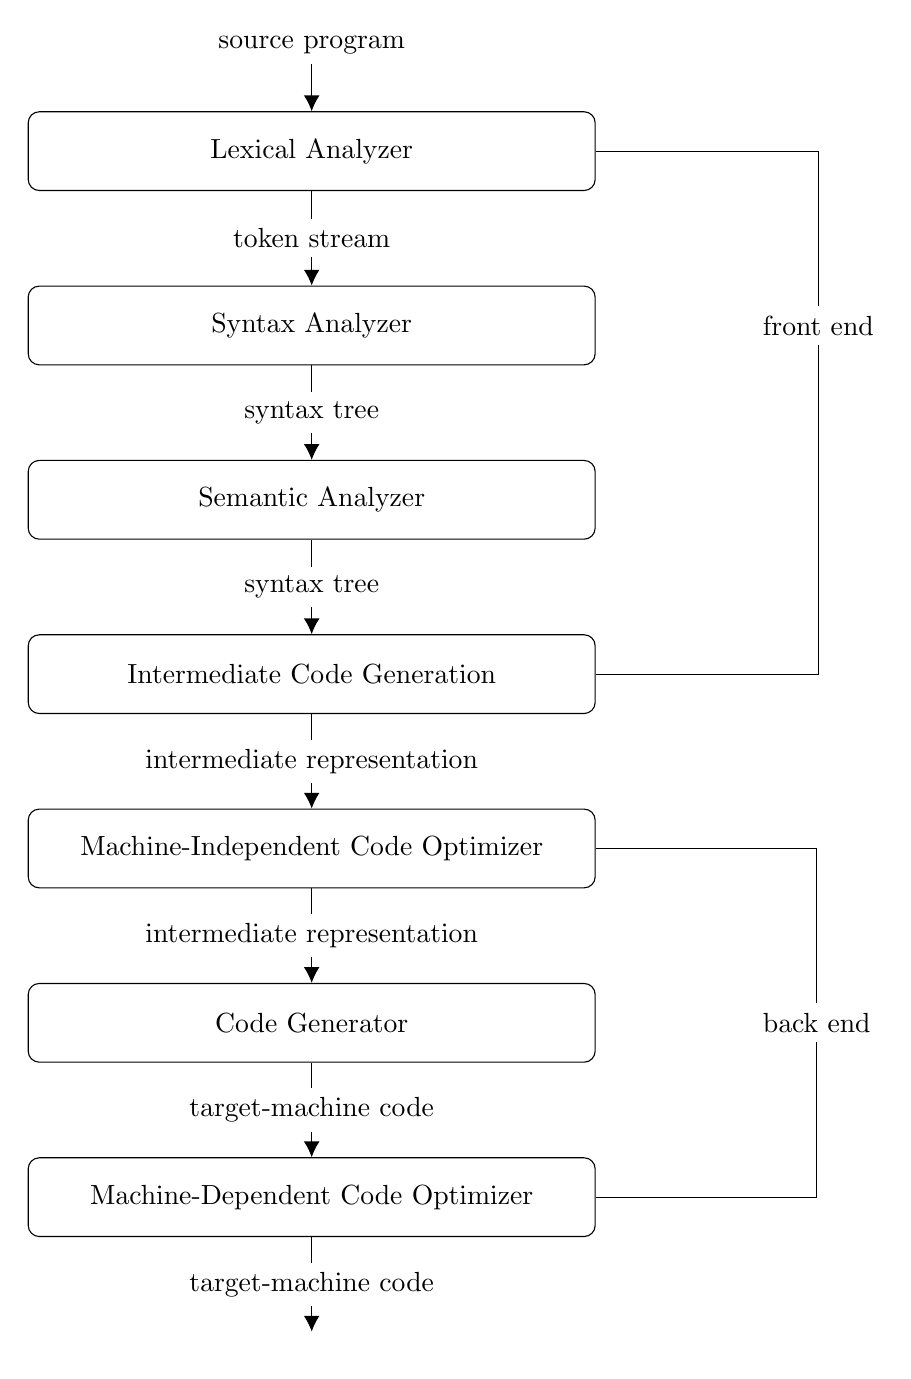
\begin{tikzpicture}[
        >={Latex[width=2mm, length=2mm]},
        ir/.style = {
                fill=white
            },
        phase/.style = {
                rectangle,
                rounded corners,
                minimum width=7.2cm,
                minimum height=1cm,
                text centered,
                draw=black,
            },
        ]
        \node (start) [ir] {source program};
        \node (lexical) [phase, below=\myflowchartlowermargin/2 of start] {Lexical Analyzer};
        \node (syntax) [phase, below=\myflowchartlowermargin of lexical] {Syntax Analyzer};
        \node (semantic) [phase, below=\myflowchartlowermargin of syntax] {Semantic Analyzer};
        \node (intermediate) [phase, below=\myflowchartlowermargin of semantic] {Intermediate Code Generation};
        \node (opt ind) [phase, below=\myflowchartlowermargin of intermediate] {Machine-Independent Code Optimizer};
        \node (codegen) [phase, below=\myflowchartlowermargin of opt ind] {Code Generator};
        \node (opt dep) [phase, below=\myflowchartlowermargin of codegen] {Machine-Dependent Code Optimizer};
        \node (end) [below=\myflowchartlowermargin of opt dep] {};

        \node (frontend) [right=2cm of syntax] {front end};
        \node (backend) [right=2cm of codegen] {back end};

        \draw [->] (start) -- (lexical);
        \draw [->] (lexical) -- node [ir] {token stream} (syntax);
        \draw [->] (syntax) -- node [ir] {syntax tree} (semantic);
        \draw [->] (semantic) -- node [ir] (syntax tree) {syntax tree} (intermediate);
        \draw [->] (intermediate) -- node [ir] {intermediate representation} (opt ind);
        \draw [->] (opt ind) -- node [ir] {intermediate representation} (codegen);
        \draw [->] (codegen) -- node [ir] {target-machine code} (opt dep);
        \draw [->] (opt dep) -- node [ir] {target-machine code} (end);
        \draw (lexical.east) -| (frontend.north);
        \draw (intermediate) -| (frontend);
        \draw (opt ind.east) -| (backend.north);
        \draw (opt dep.east) -| (backend);
    \end{tikzpicture}
    \caption{Phases of a compiler and the intermediate representations between them. Adapted from~\textcite{Aho:2006:CPT:1177220}.}
\end{figure}

According to \textcite{appel2003modern}, \textquote{An intermediate representation (IR) is a kind of abstract machine language that can express the target-machine operations without committing to too much machine-specific detail}.
The authors continue by adding that the IR \textquote{is also independent of the details of the source language}~\cite{appel2003modern}.
This means that the abstract notations exclusive to a higher-level language are handled by the front end of a compiler so that, by the time the source program is transformed into the IR, the computations described by the IR are semantic equivalent to the computations described by the source program but are now in the notations of an abstract machine language.
Although the semantics of the computations are the same, there may be semantics in the higher-level language that are not present in the IR.\@
The front end of a compiler is then responsible to check if all semantic aspects of the source program are sound to the source language specifications before the generation of the IR~\cite{Aho:2006:CPT:1177220}.
The authors explain that the checks made during compilation are called \textit{Static Checks}, and they are not only capable of assuring that the source program can be successfully compiled, but have the potential to catch programming errors early, before the program can be executed~\cite{Aho:2006:CPT:1177220}. One of the static checks executed during compilation is \textit{type checking} and is part of the semantic analysis phase of the compiler's front end~\cite{appel2003modern}.

The type checking executed during the semantic analysis phase is designed in accordance with the source language's type system.
\textcite{pierce2002types} defines a type system as: \textquote{A tractable syntactic method for proving the absence of certain program behaviors by classifying phrases according to the kinds of values they compute}.
Hence, a phrase written with higher-level notations such as
\begin{equation}\label{eq:type_example1}
    \verb+x * 30+
\end{equation}
may be classified to compute a value of type \verb+Integer+, written
\begin{equation*}
    \verb+x * 30: Integer+
\end{equation*}
meaning that~\ref{eq:type_example1} is a phrase that computes a mathematical integer value.
As a counter example, if defined by the type system that the multiplication between a value of type \verb/Character/ and a value of type \verb/Integer/ was not allowed, and we had both classifications
\begin{equation*}
    \verb/x: Character/ \quad \textrm{and} \quad \verb/30: Integer/
\end{equation*}
the phrase in~\ref{eq:type_example1} would be semantically unsound and should be indicated as a type error by the type checker.

According to \textcite{jhala2020refinement} type systems are mainly used to describe valid sets of values that can be used for different computations, so that the compiler can eliminate, during its execution, a variety of possible run-time errors during the target program execution.
Type systems like the ones used by popular modern programming languages such as C\#, Haskell, Java, OCaml, Rust and Scala have similar kinds of rules and are the most widespread tool used to guarantee the correct behavior of a program~\cite{jhala2020refinement}.
In \textcite{jhala2020refinement}, the authors affirm that, although type systems are widespread and effective, well-typed programs do go wrong; and goes on to describe a few wrong behaviors that are common to the most popular type systems. Within them, we have:
\begin{itemize}
    \item \textbf{Division by zero:} Constraining the types of the division operation to \verb/int/ does not protect the program to execute a division by zero at run-time; also, it does not guarantee that the arithmetic operations will not under- or over-flow~\cite{jhala2020refinement}.
    \item \textbf{Buffer overflow:} Constraining the index of the access of a \verb/array/ or \verb/string/ to \verb/int/ does not protect the program to try to access data from beyond the data structure's end~\cite{jhala2020refinement}.
\end{itemize}

An effort can be made while designing a type system so that they can further restrict the values of certain types.
We can be extended a type system to further \textit{refine} its types with logic predicates and this method is called \textit{Refinement types with predicates}~\cite{jhala2020refinement}.
It allows programmers to constrain existing types by using predicates to assert desired properties of the values they want to describe~\cite{jhala2020refinement}.
For example, while \verb/int/ types can assume any integer values, we can write the refined type
\begin{equation*}
    \verb/type nat = int[v | 0 <= v]/
\end{equation*}
where the newly defined type \verb!nat! will only be able to assume positive integer values.
Alone, this refinements may seam a just a gimmick, but combined with function the programmer can describe precise contracts that describe the functions legal inputs and outputs~\cite{jhala2020refinement}.
For example, the author of an \verb!array! library may specify the functions signatures types
\begin{equation*}
    \begin{aligned}
         & \verb/fn size: x:array(a) -> nat[v | v = length(x)]/ \\
         & \verb/fn  get: x:array(a) -> nat[v | v < length(x)] -> a/
    \end{aligned}
\end{equation*}
where \verb!size! and \verb!get! are functions and \verb!x! is the name of the first variable.
In this type system, a call to \verb+size(arr)+ returns a value $s$ of type \verb!nat! constrained to a single value equal to the length of \verb!arr!; hence, the type of $s$ constrains $s$ to the exact length of \verb+arr+.
Furthermore, a call to \verb+get(arr, i)+ requires the index \verb+i+ to be within the bounds of \verb+arr+.
Given these definitions, the refinement type checker can then prove, during the analysis phase (i.e.\ at compile-time), that the contracts of both \verb+size+ and \verb+get+ will not be violated, ensuring all array access to be sated when executing the target program (i.e.\ at run-time).

\section{Goals}\label{chapter:introduction:sec:goals}

The primary goal of this work is to answer the following question: Which opportunities for code optimization arrive from compiling a higher-level language with refinement types during intermediate code generation that are not possible without refinements types?

For that we will be designing a language called \textit{Ekitai}.
Designing a new language is particularly advantageous because we have full control of all the language features being implemented and allow us to build the language, the refinement type system, and the intermediate code generation, one feature at a time.

\subsection{Specific Goals}
The specific goals of this work are to:
\begin{itemize}
    \item Design a programming language;
    \item Design the programming language's type system with refinement types using operational semantics;
    \item Implement a compiler's front for the designed language including:
    \begin{itemize}
        \item A lexical analyzer;
        \item A syntactic analyzer for the language's syntax;
        \item A semantic analyzer with a type checker for the language's type system;
        \item An intermediate code generator;
    \end{itemize}
    \item Find optimization opportunities during intermediate code generation.
\end{itemize}

\section{Methodology}

The aim of this work is to find optimizations opportunities during intermediate code generation of a higher-level language with refinement types. In order to achieve our goals we conducted applied exploratory research were we employed an engineering-oriented research methodology together with literature research to build the compilers front end.

\section{Structure of the work}

We will present here the structure of this work.

\chapter{Background}\label{chapter:background}

In this chapter we will present the background needed to build a compiler and create an operational semantic for the refinement type system.

\subsection{Lexical Analysis}

The first phase of a compiler is called lexical analysis, or \textit{scanning}.
The lexical analyzer will read a stream of characters from the source program and group the characters into sequences called \textit{lexemes}.
For each lexeme, the lexical analyzer generate a \textit{token} with different meta-data depending on the token type.
For example, analysing the following program:
\begin{quote}
    \begin{verbatim}
let a = b + 60 / c
\end{verbatim}
\end{quote}
A lexical analyzer may output the following token stream:
\begin{quote}\label{figure:introduction_token_stream}
    \begin{verbatim}
<let> <id, a> <=> <id, b> <+> <number, 60> </> <id, c>
\end{verbatim}
\end{quote}
Where tokens are of the form \verb+<token-type, meta-data>+, when no meta-data is needed it can be omitted from the token notation.
We can see that this lexical analyzer decided to map the lexemes `let', `=', `+' and `/', to the respective tokens \verb+<let>+, \verb+<=>+, \verb-<+>- and \verb+</>+;
the lexemes `a', `b' and `c', to the respective tokens \verb+<id, a>+, \verb+<id, b>+, and \verb+<id, c>+, which all have the same token type `id' and carry as meta-data the lexeme that generated the mapping; and the lexeme `60', to the token \verb+<number, 60>+, which has token type `number' and has the its value of $60$ as meta-data.
\subsection{Syntax Analysis}

The second phase of a compiler is called syntax analysis, or \textit{parsing}.
The \textit{parser} then receives as input a token stream produced by the lexical analyzer and creates a tree-like intermediate representation that is constrained by a particular grammatical structure.

% We can then build a parser $p$ for the following gammar in BNF notation:
% \begin{quote}
% \begin{verbatim}
% <let-statement> ::= let id = <expr>
% <expr> ::= <term> + <expr> | <term>
% <term> ::= <term> / <factor> | <factor>
% <factor> ::= id | number
% \end{verbatim}
% \end{quote}
% where we define productions of the type $symbol ::= expression$

If we give the token stream from Section~\ref{figure:introduction_token_stream} as input to a parser it may output the tree structure found on Figure~\ref{figure:introduction_ast}.
This structure already has more information than the linear token stream it received as input.
For example, it is prepared in such a way to preserve the order of operations from classic arithmetic, the tree has an interior node labeled $/$ with \verb+<number, 60>+ as its left child and \verb+<id, c>+ as its right child making it explicit that we must first divide $60$ by $c$ before evaluating the interior node labeled $+$ which depends on the result of $/$ as its right child.

\begin{figure}
    \caption{A possible parser output for the token stream from Section~\ref{figure:introduction_token_stream}}\label{figure:introduction_ast}
    \centering
    \begin{tikzpicture}
        \node (is-root) {=}
        [sibling distance=2cm]
        child { node {<id, a>} }
        child {
                node {+}
                    [sibling distance=2cm]
                child { node {<id, b>} }
                child {
                        node {/}
                            [sibling distance=2.2cm]
                        child { node {<number, 60>} }
                        child { node {<id, c>} }
                    }
            };
    \end{tikzpicture}
\end{figure}

\subsection{Semantic Analysis}

The third phase of a compiler is called semantic analysis.
It is responsible to use the tree structure generated by the parser to check if the source program is semantically consistent with the language specification.
An important part of semantic analysis is \textit{type checking} where it will try to validate the program to the language specification's type system.

If we feed a type checker with the tree structure presented on Figure~\ref{figure:introduction_ast}.
It may make use of a symbol table containing the type information of the identifiers `b' and `c' to type check all nodes of the tree for consistency.
Suppose a symbol table that maps the identifier `c' to the type `boolean', written `\verb+c: boolean+', which would compose of the values `true' and `false'.
With this information, the type checker would be able to decide if the operation `\verb+60 / c+' is semantically sound to the language's type system.
Does the language type system specifies as valid to divide a number by a boolean?

\alcides{A partir daqui é o que faz sentido estar na introdução: identificar que tipos de erros são apanhados pelos typesystems, e indicar que existem sistemas de tipos mais avançados, onde podemos especificar predicados. Dar dois ou três exemplos. O resto pode ir também para background.}

If it does, what does it mean to divide the value 60 by `false'?
Maybe, whoever designed the language decided that if the dividend is a value of type number and the divisor is a value of type boolean, it will use some rule to convert the divisor's type to number in order to keep the program semantically sound.
Maybe, the language's type system forbids this behaviour and will halt the compilation process with some error message.
This are decisions made when building a language's type system.


\begin{itemize}
    \item \textbf{Division by zero:} Constraining the types of the division operation to `int' does not protect the program to execute a division by zero at run-time.
          Also, it does not guarantee that the arithmetic operations will not under- or over-flow.
    \item \textbf{Buffer overflow:} Constraining the index of the access of a `array' or `string' to `int' does not protect the program to try to access data from beyond the data structure's end.
    \item \textbf{Logic bugs:} The type system of modern languages allow for the creation of custom types like \verb+structure date { day: int, month: int, year: int}+, where its values are compound of three `int' values for day, month and year.
          But the type `date' can not guarantee that the value for day will be valid for a certain value of month and year.
    \item \textbf{Correctness errors:} The type system can guarantee that a sorting procedure will produce a value of type list  but can not guarantee that the list was, in fact, sorted.
\end{itemize}

A type system can be extended to further \textit{refine} its types with logic predicates.
This method is called \textit{Refinement types with predicates}.
It allows programmers to constrain existing types by using predicates to assert desired properties of the values they want to describe.
For example, while `int' types can assume any integer values, we can write the refined type
\begin{quote}
    \begin{verbatim}
type nat = int[v | 0 <= v]
\end{verbatim}
\end{quote}
where `nat' will only be able to assume positive integer values.
Alone, this refinements may seam a just a gimmick, but combined with function the programmer can describe precise contracts that describe the functions legal inputs and outputs.
For example, the author of a array library may write the functions
\begin{quote}
    \begin{verbatim}
val size: x: array(a) -> nat[v | v = length(x)]
val get: x: array(a) -> nat[v | v < length(x)] -> a
\end{verbatim}
\end{quote}
which guarantees that a call to \verb+size(arr)+ returns a value with the exact length of \verb+arr+, and that a call to \verb+get(arr, i)+ requires the index \verb+i+ to be within the bounds of \verb+arr+.
Given this definitions the refinement type checker can then prove, during the analysis phase (i.e.\ at compile-time), that the contracts of both \verb+size+ and \verb+get+ will not be violated, ensuring all array access to be sate when executing the target program (i.e.\ at run-time).

Refinement types offer the option to add information to the type system about the invariants and correctness properties a programmer may care about.
It is done in such a way that, if the programmer desires, no refinement needs to be added and can be thought like a typical type system.
On the other hand, programmers can incrementally add refinements to ensure important properties about the source program.
They could begin with basic safety requirements, e.g.\ eliminating division by zero and buffer overflow, or guarantee that a function does not receive a empty collection, and then incrementally add to the specification invariants of custom data types.
Ultimately going all the way to specifying and verifying the correctness of different procedures at compile-time.
By enabling verification on the same language as the programming language, refinement types bridge implementation and prof together.
This approach creates a development cycle were the implementation hits programmers to what properties are important to verify, and the verification hits on how the implementation can be restructured to better express the invariants and enable formal proof.


\chapter{Related Work}\label{chapter:related_work}

In this chapter we will present prior work related to refinement types and llvm.

\chapter{TODO:proposal}

In this chapter we will present the built language and type system.

%%%%%%%%%%%%%%%%%%%%%%%%%%%%%%%%%%%%%%%%%%%%%%%%%%%%%%%%%%%%%%%%%%%%
%%% Elementos pós-textuais                                       %%%
%%%%%%%%%%%%%%%%%%%%%%%%%%%%%%%%%%%%%%%%%%%%%%%%%%%%%%%%%%%%%%%%%%%%

\postextual{}
\printbibliography{}

\end{document}
